\documentclass[12pt,a4paper]{article}
\usepackage{better_poster}
\usepackage[hidelinks]{hyperref}

% ---- fill in from here

% authors
\title{}
%\author{Lana Sinapayen, Someone Else}

% type of poster: [exp]erimental results, [methods], [theory]
% Disclaimer: the original classification had "study" and "intervention" as separate categories. I group them under experimental results.
\newcommand\postertype{exp} % [exp],[methods],[theory]

\begin{document}

% main point of your study
\makefinding{\textbf{Martin Ladecký}
}

%%  č.\textbf{14.} \\
%\normalsize{do studentské komory}\\
%AS FSV ČVUT 
% \makemain{
% }{

% }


% the main text of your poster goes here
\makemain{
    % you can have 1 or 2 columns
   % \raggedcolumns
  %  \begin{multicols}{1}
  \vspace{-1.5cm}
    	        \section*{Chci prosazovat:}
    	        
    	\begin{itemize}
    	\large{
    		\setlength\itemsep{0.5em}
    		\item \textbf{Zapojení studentů do výzkumných projektů}
    		\item \textbf{Rozšíření FIT klubu a sportovních možností} 
			\item \textbf{Funkční eduroam na celé fakultě} 
    		\item \textbf{Zřízení kuchyňského koutku pro studenty}
    		\item \textbf{Prohlubování zapojení počítačů do výuky}
    		\item \textbf{Zodpovědné a transparentní hospodaření} 
    	    \item \textbf{Podpora spolupráce mezi katedrami}}
    	\end{itemize}
    % \vspace{0.5cm}
        \section*{Něco o mně}
        \begin{itemize}
        \setlength\itemsep{0.1em}
            \item Jsem doktorand na katedře matematiky a současně pracuji jako výzkumný pracovník na katedře mechaniky naší fakulty. Rád sportuji, cestuji a baví mě věda.
            
            \item Jako student vím, že pro dobré studijní výsledky je důležitá psychická i fyzická pohoda. Chci, abychom se na fakultě cítili dobře a měli kde sportovat.
            
            \item Využívání moderních technologii při studiu je v dnešní době nevyhnutelné. Stabilní WIFI připojení by mělo být samozřejmostí.
            
            \item Během svého působení jsem pracoval na mnoha výzkumných projektech a vím, jak důležitá je mezioborová spolupráce. Proto bych chtěl podporovat dobré vztahy mezi katedrami.
            
            \item Záleží mi na férovém fungovaní naší fakulty, a proto chci  dohlížet na zodpovědné a transparentní hospodaření.
            
		
        \end{itemize}
        

  %%%      
    % this determines where your columns will be separated

    
  %  \end{multicols}
}
% If you have extra figures or data to show
\makeextracolumn{
    
    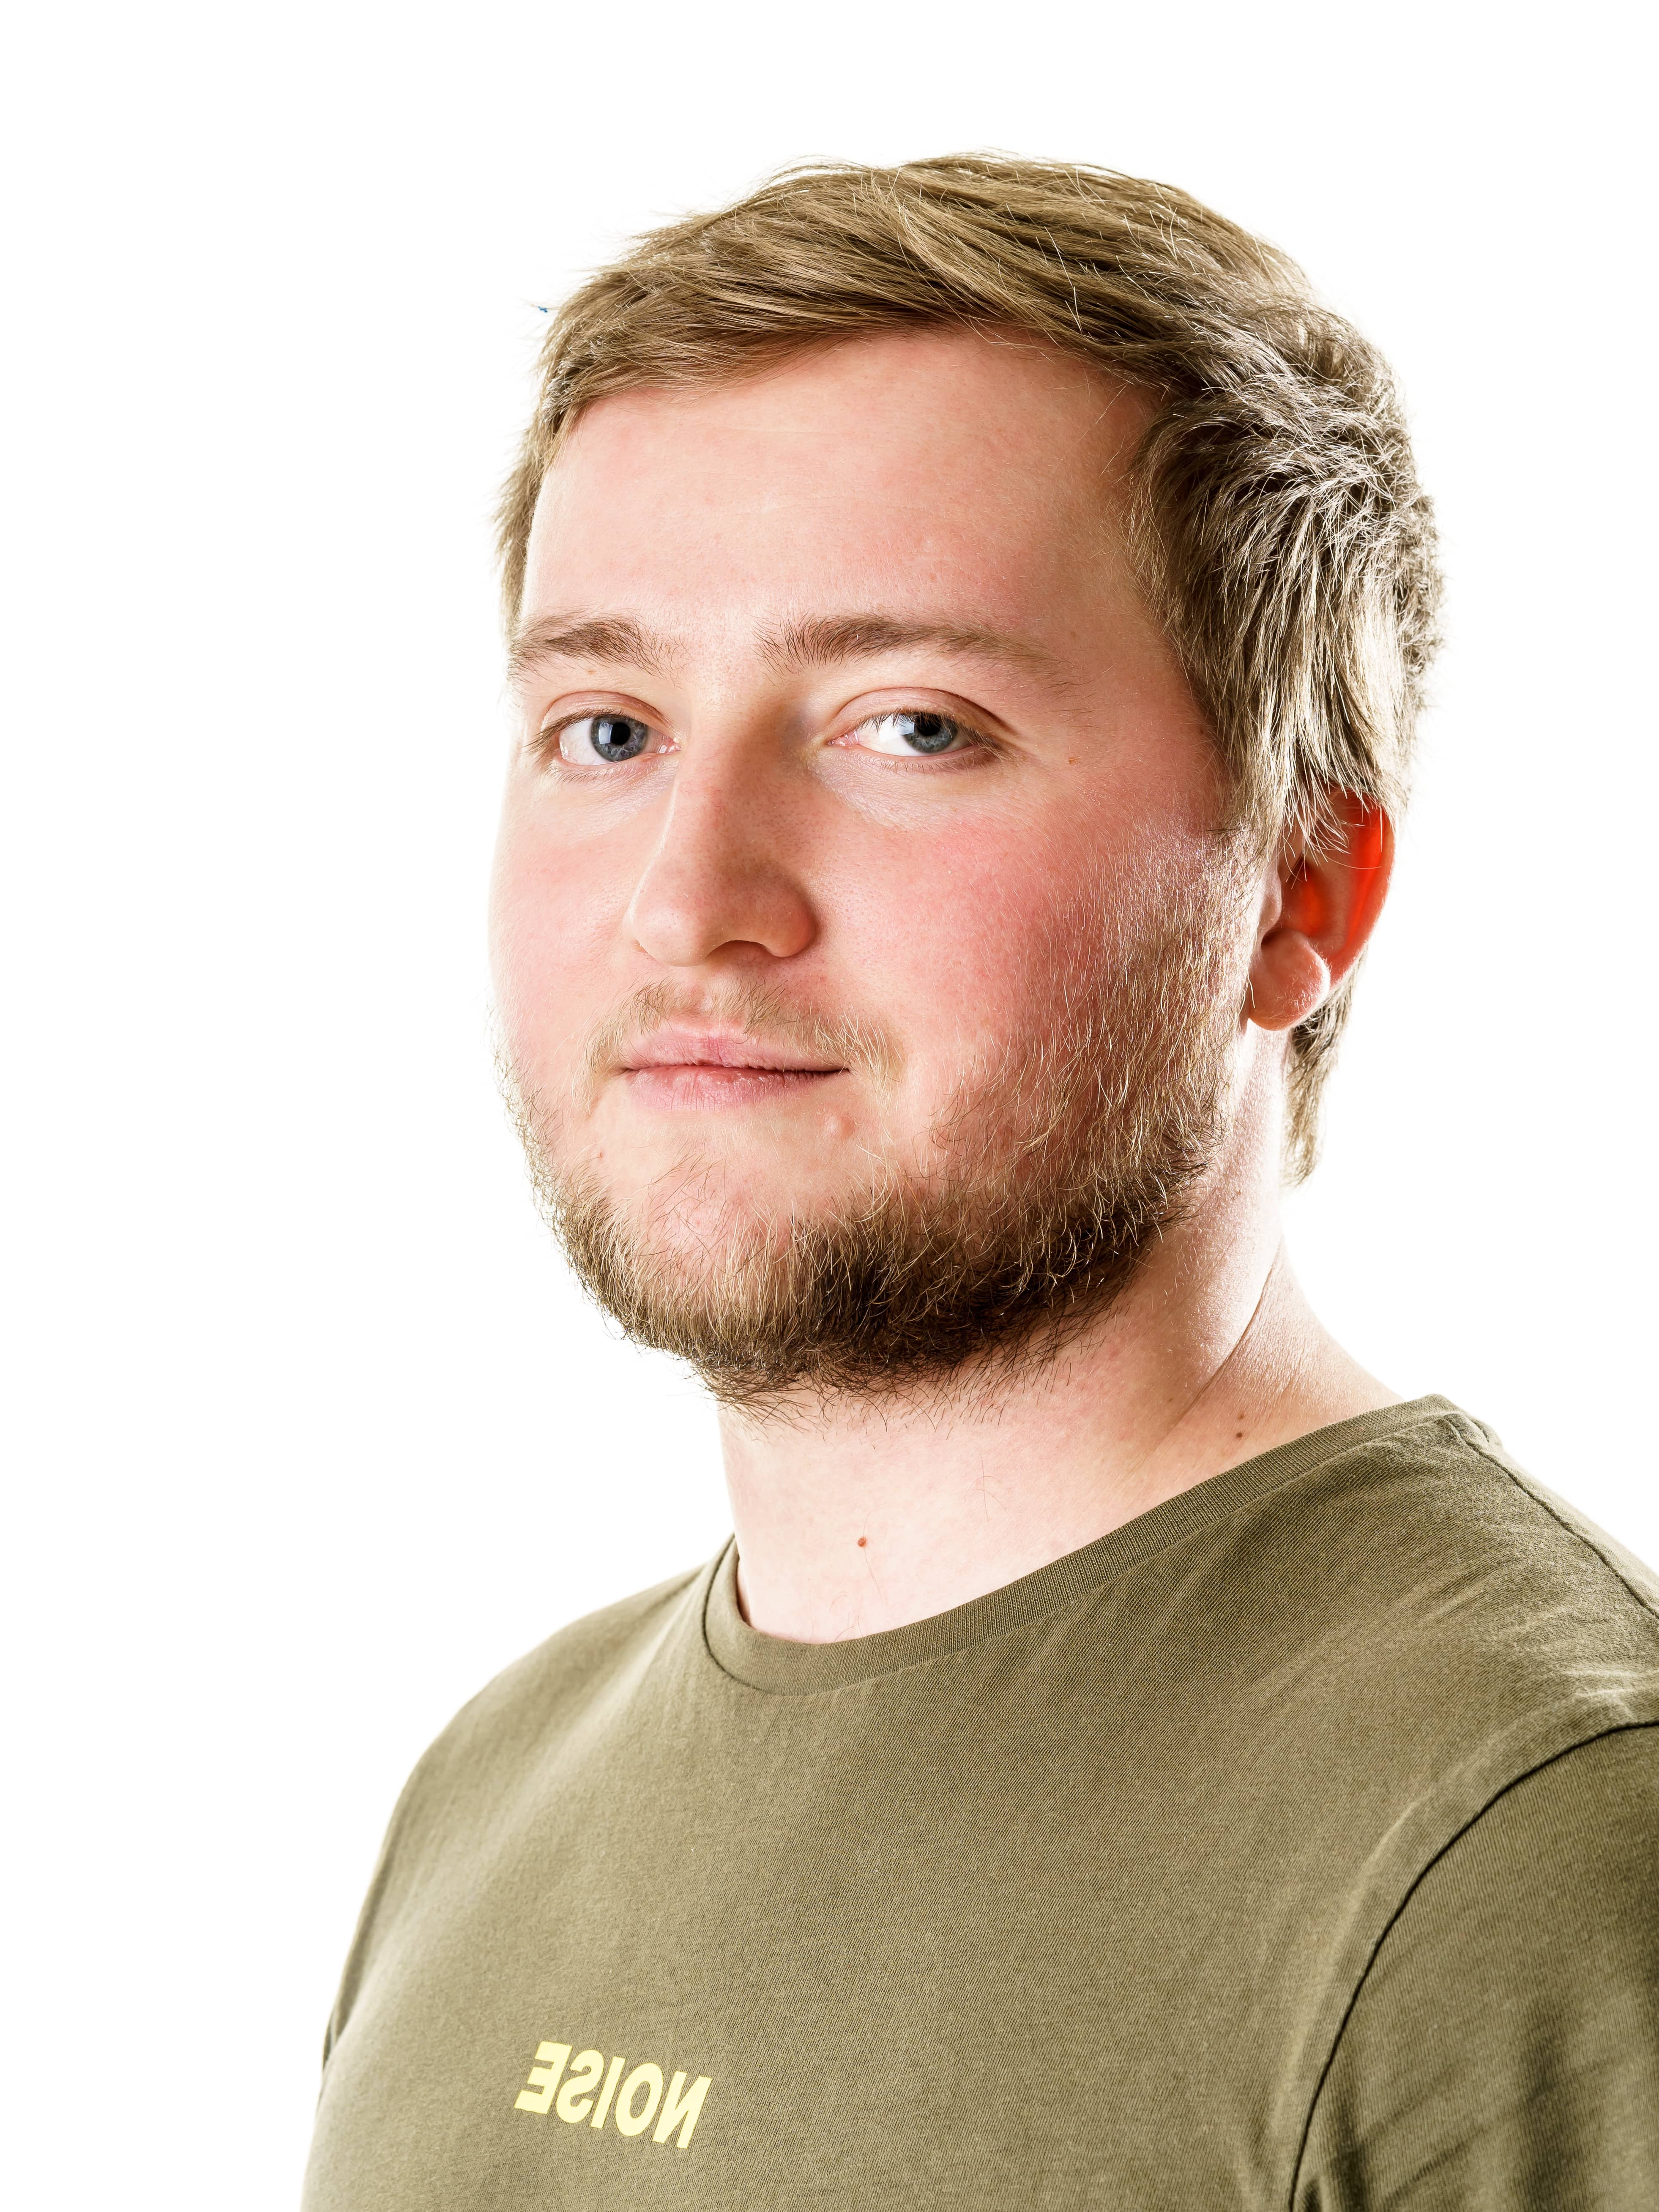
\includegraphics[width=1\linewidth]{images/photo_ML.jpg}
  %  \includegraphics[width=0.5\linewidth]{}
    
    \begin{itemize}
    \setlength\itemsep{0.1em}
    \large{
    	\item 25 let
        \item Doktorand
        \item Výzkumný pracovník
        \item Místnost B-302
        \item \href{martin.ladecky@fsv.cvut.cz}{martin.ladecky@fsv.cvut.cz}
    \vspace{2cm}   
    \item  Neváhejte mě kontaktovat s jakýmikoli dotazy :)
   	} 
    \end{itemize}
}

% footer
% generate qr code from https://www.qr-code-generator.com/ and replace qr_code.png
% default: barcode on the left
\makefooter{images/logo_FSv_zkratka.jpg}{images/symbol_cvut_plna_verze.jpg}

% replace with this like for barcode on the right
%\makealtfooter{images/uni_logo.png}{images/qr-code.png}
 
\end{document}